\chapter{System design}
In this chapter I'm introducing the initial design of the above mentioned system from both hardware and
software aspects. Since there are several unknown factors 
during this phase, the designs described in this chapter are presented as initial designs. The actual
system design will be based on the experience gained during several trial-and-error based iterations
in simulations.

Multiple aspects need to be taken into account to determine the number and the placement of the LIDAR sensors.
The specifications of the LIDAR and the characteristics of SLAM algorithms also drive these aspects. 
Higher sampling rate can be achieved by placing multiple sensors close to each other in a way that 
their scanned trajectories overlap. The resolution needed by the chosen SLAM algorithm also affects 
the number and placement of the sensors, the resolution can be increased by programmatically narrowing
down the field of view of the LIDAR.

Quadcopters have a natural tendency to increase their pitch and roll angles when moving around 
on the horizontal plane. By determining the characteristic pitch and roll angles during an indoor flight,
the placement of the sensors can be refined. This way fewer LIDARs are needed for scanning the
whole range. Using fewer sensors is beneficial, it reduces complexity in hardware and software too.
While during simulations we don't need to worry about physically attaching the sensors on the frame or even
supplying power to them, in a real implementation these might be limiting factors.

On a real drone LIDAR measurements cannot be sent straight to ROS topics, because a low level communication needs
to be established to configure and read out measurements from the sensors. There needs to be a device that 
handles communication with the sensor and forwards messages to ROS topics.
This device can be the Pixhawk 4 autopilot board using a custom firmware or a custom built hardware 
independent from the autopilot board or a combination of these two.

\section{Pixhawk 4}
Pixhawk 4 is an advanced autopilot designed by the collaboration of Holybro and PX4 team \cite{Pixhawk4Website}. 
It is optimized to run the official PX4 flight stack. Because of its modular-, open-design and open-source 
firmware, it is a good choice for rapid development and academic purposes. Its modularity comes from the 
connectors on the top of the device that are used to supply power for the board, output PWM signal for 
the motors and to add peripherals like GPS antenna, telemetry or integrate custom devices using available
bus connectors. 

When moving to real world applications, the PX4 SITL flight stack seen on the most left block on figures
\ref{fig:px4_sitl_simulation} and \ref{fig:px4_sitl_ros_wrapper}, is to be replaced by the Pixhawk 4 board.

\begin{figure}[h]
    \centering
    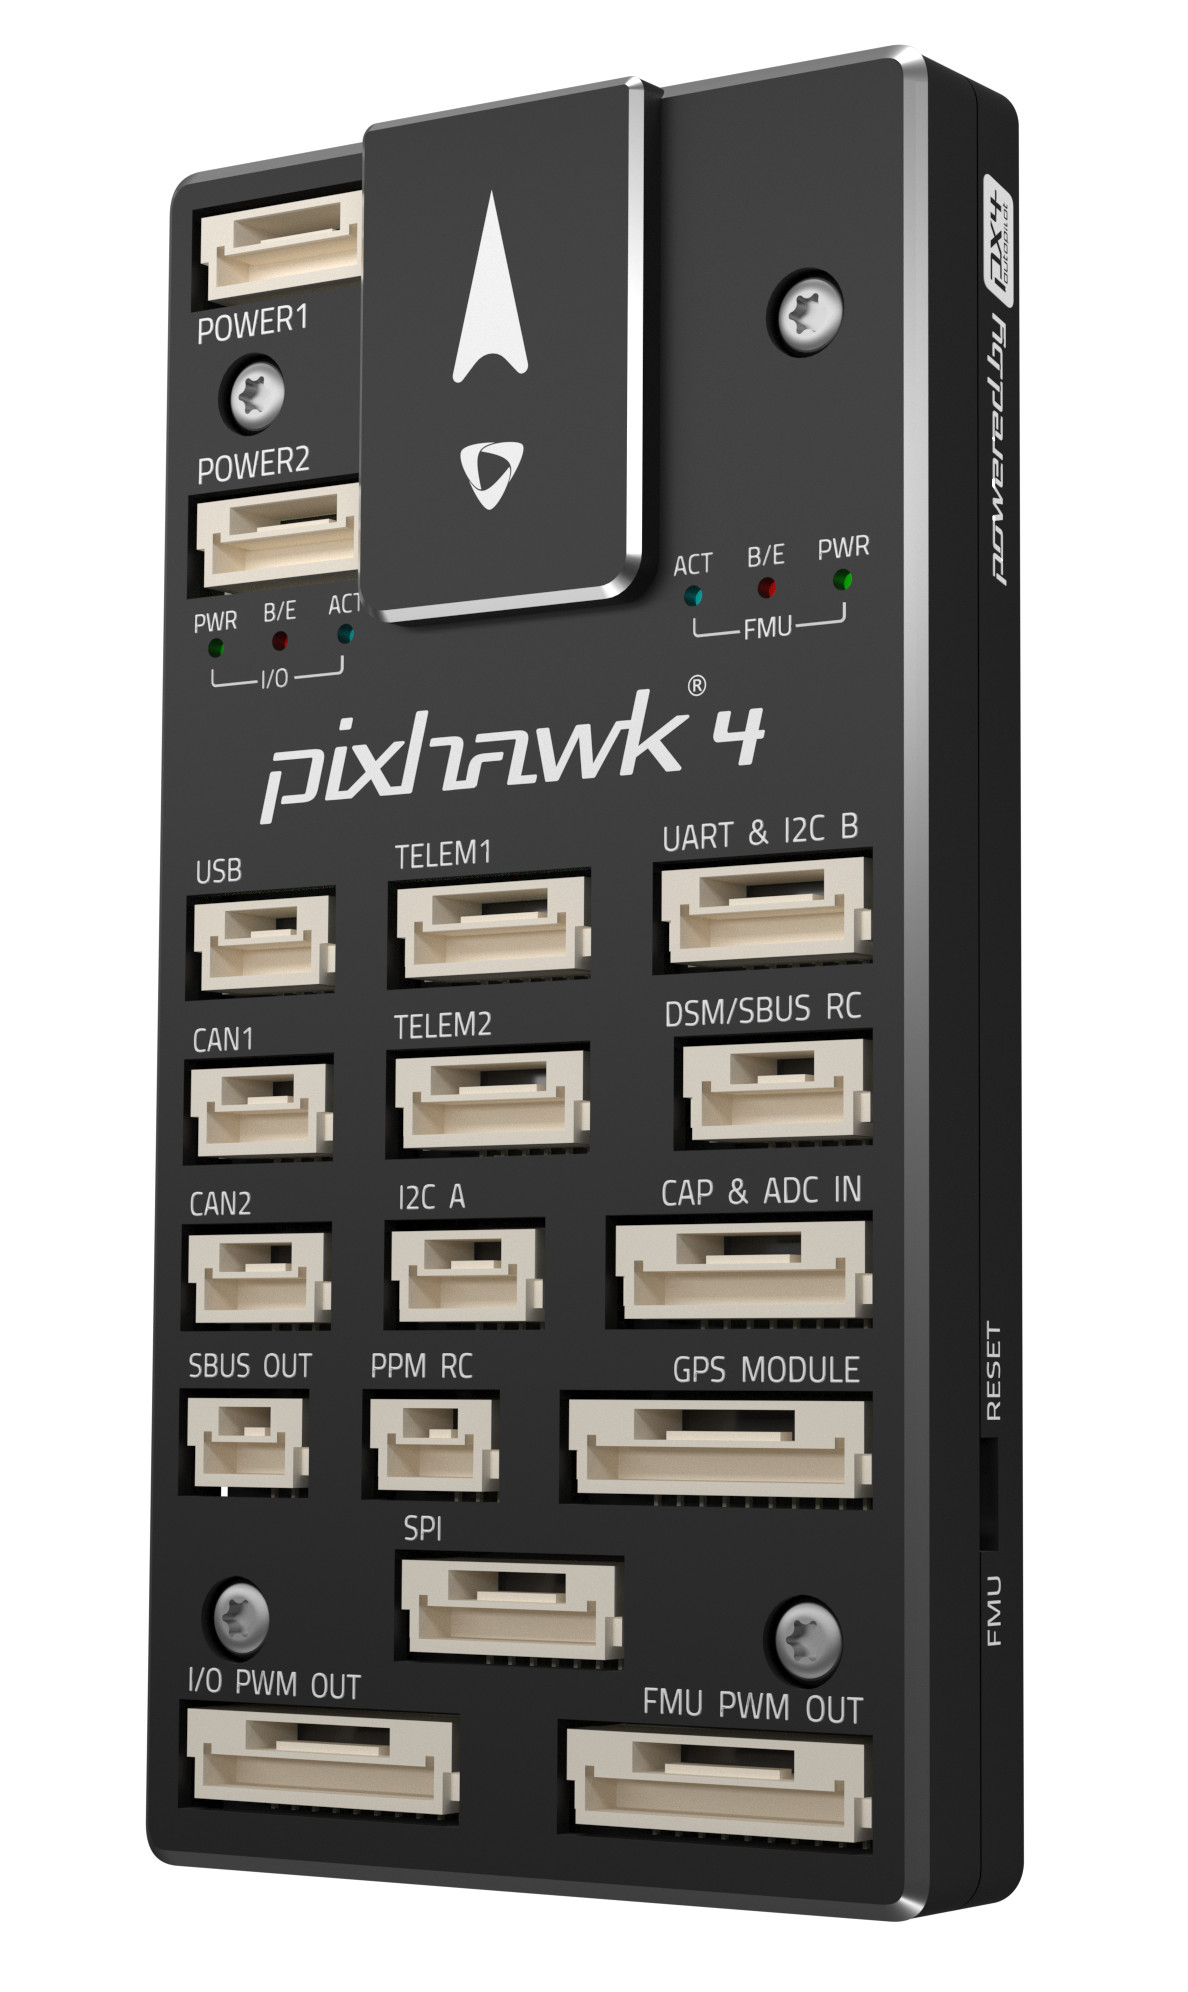
\includegraphics[width=25mm, keepaspectratio]{figures/pixhawk4.jpg}\hspace{0cm}
    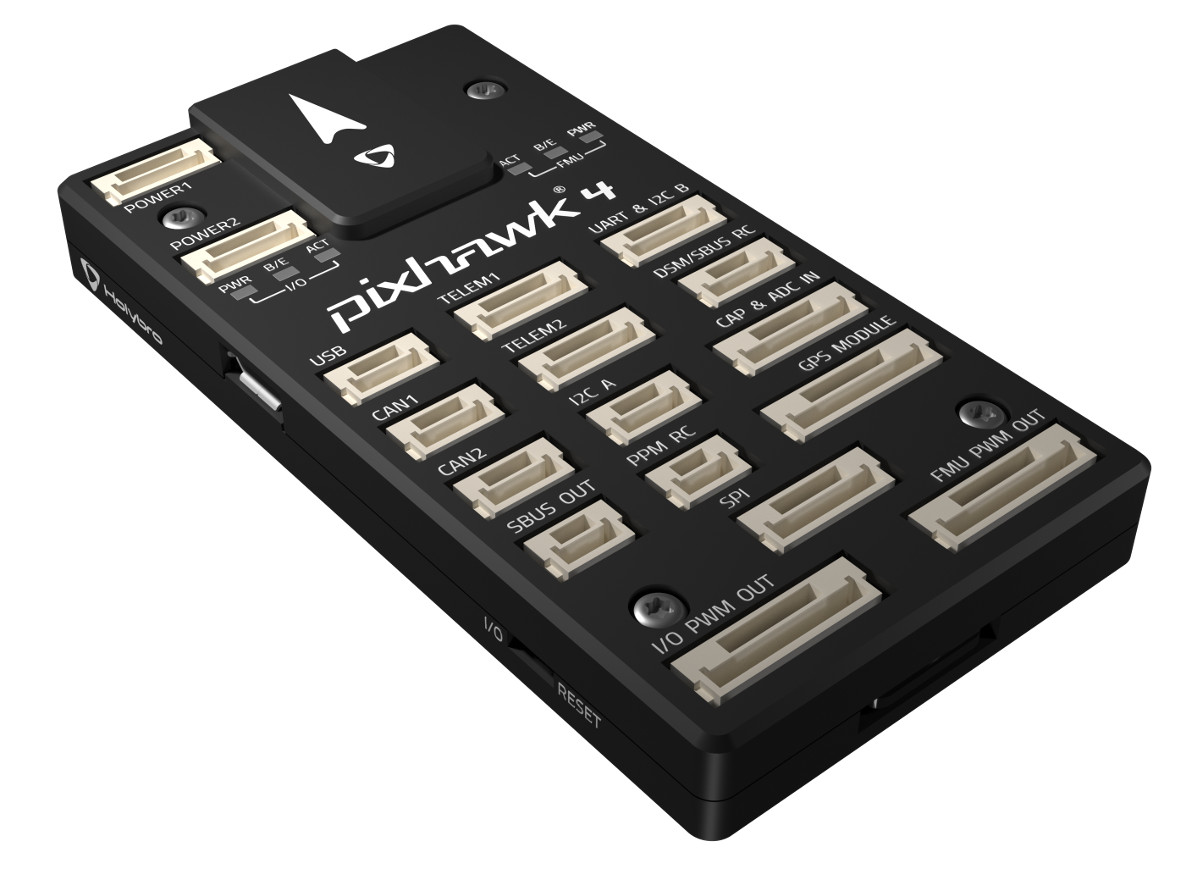
\includegraphics[width=50mm, keepaspectratio]{figures/pixhawk4_2.jpg}
    \caption{Pixhawk 4 advanced autopilot}
    \label{fig:px4_sitl_ros_wrapper}
\end{figure}

\section{VL53L1X LIDAR sensor}
VL53L1X is a long distance ranging Time-of-Flight sensor produced by STMicroelectronics \cite{VL53L1XDatasheet}. 
The size of the module is 4.9x2.5x1.56mm, it emits 940nm invisible laser and uses a SPAD(single photon 
avalanche diode) receiving array with a field of view of 27$^{\circ}$. The module runs all digital signal
processing on a built in low power microcontroller that frees up the host processor from these tasks.
The sensor according to the datasheet is capable of 50Hz ranging frequency and up to 400cm distance 
measurements. The laser receiving array's size can be programmatically changed by setting 
region-of-interest(ROI) size. This way the sensor provides multizone operation and a higher resolution than
by using the whole SPAD array.

\begin{figure}[ht]
    \centering
    $\vcenter{\hbox{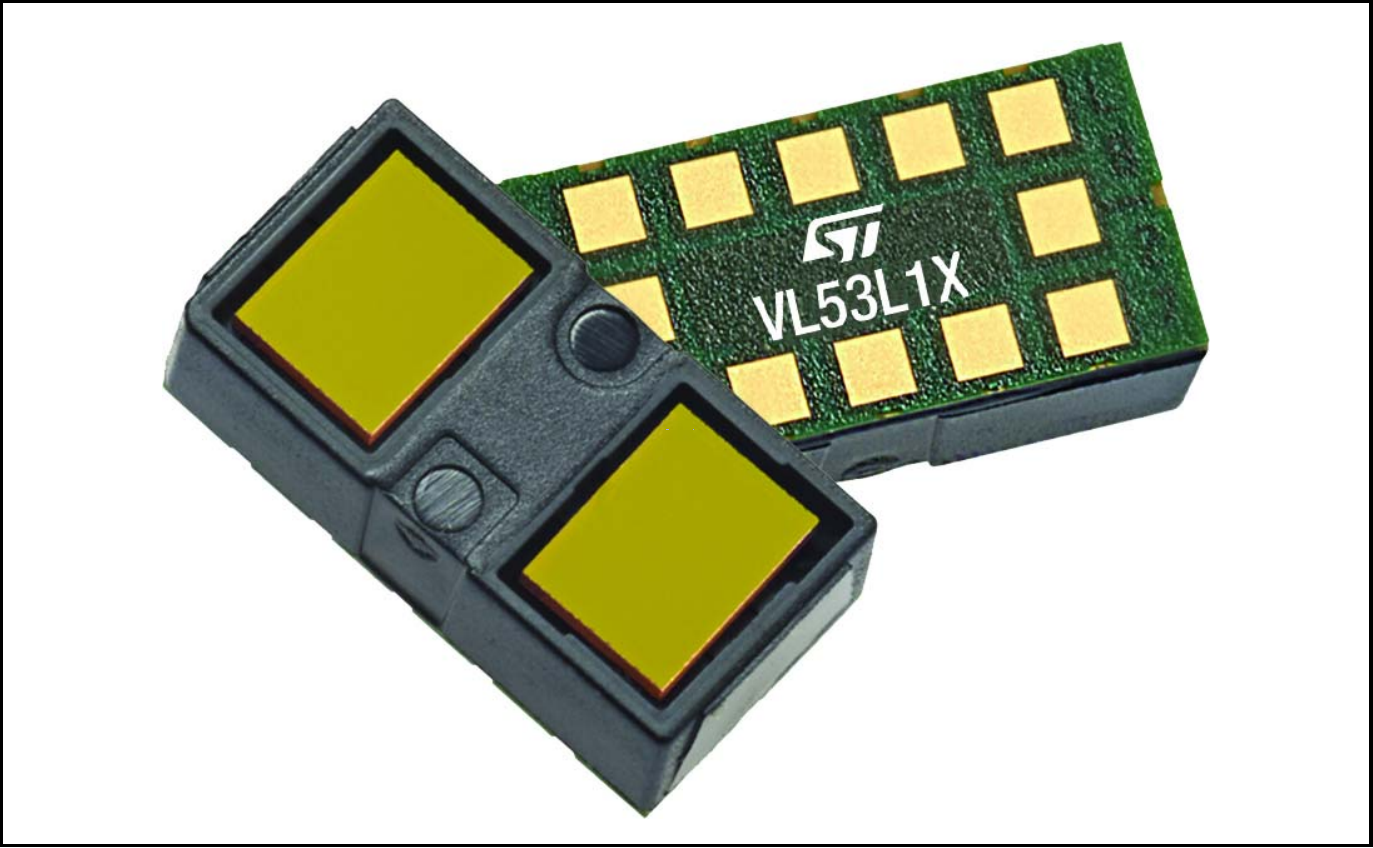
\includegraphics[width=50mm, keepaspectratio]{figures/vl53l1x.png}}}$
    $\vcenter{\hbox{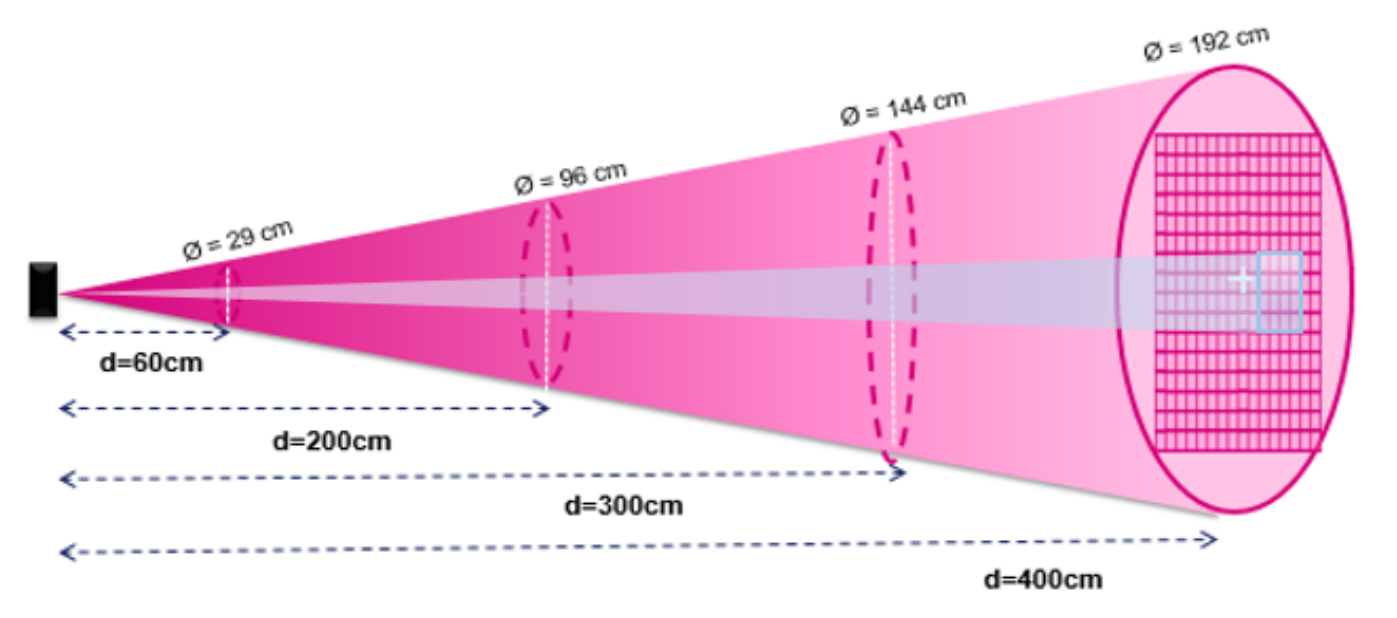
\includegraphics[width=95mm, keepaspectratio]{figures/vl53l1x_roi.png}}}$
    \caption{VL53L1X sensor \cite{VL53L1XDatasheet} and region-of-interest \cite{VL53L1XApplicationNote}}
    \label{fig:VL53L1X_sensor}
\end{figure}

I chose to use this sensor for prototyping, because of its small size, availability, low hardware 
infrastructure needs and previous experience. 


\section{LIDAR layout design}
As mentioned before, multiple aspects need to be taken into account when placing LIDAR sensors onto a
quadcopter and use the measurements for 3D SLAM. There are several parameters of the sensor that are 
highly affecting the quality of the map built by SLAM algorithms. These are the field of view, the 
sampling frequency and the maximum distance that it can measure. To better understand the effects of
these parameters it is reasonable to first reduce complexity and build a system for 2D mapping. Based on 
the experience gained during this experiment it can be better estimated how many sensors are needed for
3D SLAM. Also a possible outcome is that VL53L1X is not suitable for this purpose and a different
sensor needs to be used, with more suitable parameters.

\subsection{Layout design for 2D SLAM}
To have the best possible layout without overlapping scans, 360$^{\circ}$ of the horizontal plane 
needs to be covered by the field of view of the LIDAR sensors. The field of view of VL53L1X is 27$^{\circ}$,
so altogether 13 sensors are needed to cover 97.5\% of the plane, with 27.69$^{\circ}$ in between, leaving
only 9$^{\circ}$ of dead zone.

\begin{figure}[ht]
    \centering
    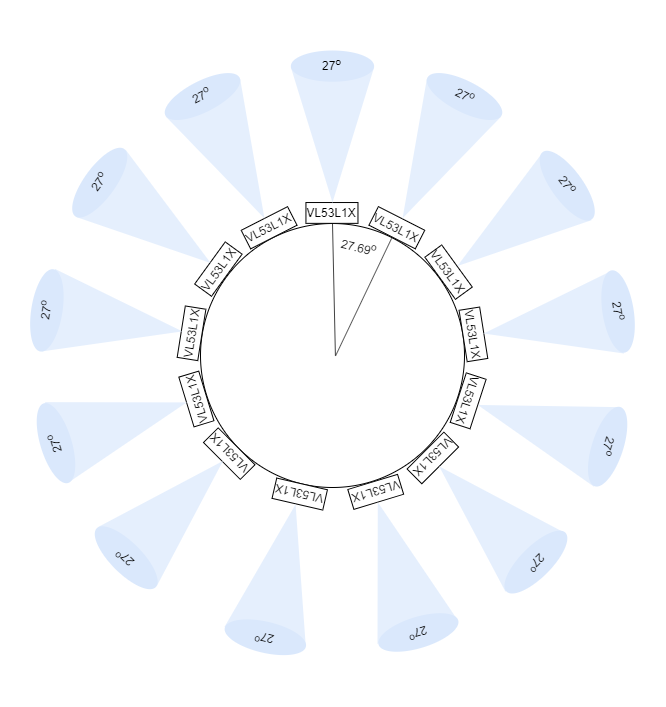
\includegraphics[width=70mm, keepaspectratio]{figures/2d_slam_13sensors.png}
    \caption{Layout of 13 LIDAR sensors}
    \label{fig:2d_13sensor_layout}
\end{figure}

In this layout the scanning on the horizontal plane is done purely by evenly placing the sensors 
around the vertical axis and doesn't take advantage of the movement of the drone during flights. 
Especially turns around the vertical axis. The usage of 13 LIDAR sensors just for 2D scanning would mean 
a lot of overhead when stepping up to 3D, so a more optimal solution needs to be found, that takes
advantage of the movement of the drone during turns and therefore uses fewer sensors. 

The lower limit for the number of sensors is what can be seen on the solution of Bitcraze, 
the Multi-ranger deck\cite{BitcrazeMultirangerDeck} uses 4 sensors on the horizontal plane facing forward, 
backwards, left and right. In their demonstration video, the map of a simple room is built in 
about 20 seconds with update rate of about 10Hz per sensor. 

\subsection{Layout design for 3D SLAM}
The layout for 3D SLAM depends on the experience gained during simulations of 2D SLAM. In 3D layout,
the pitch and roll angle changes need to be taken into account too. These differ from vehicle to vehicle,
faster drones can have a pitch of 30$^{\circ}$, but in indoor environment nor pitch nor roll will go above
15$^{\circ}$. 

\section{LIDAR data collection}
On a real drone configuration of LIDAR sensors and measurement forwarding to ROS need to be solved. 
There needs to be a device that communicates with the VL53L1X LIDAR sensors using I2C communication 
protocol and forwards messages to a ground station that handles data collection and processing.

The data collector device needs to be fast enough to keep up with the pace of 10-20 sensors,
each with a maximum of 50Hz update rate. The distance data from VL53L1X sensor consists of 12bytes, 
so 20 sensors on 50Hz generate about 12kb of data per second. This load is calculated using the 
effective data size, but on the I2C bus other messages need to be sent to trigger data read,
which means even higher load.

To evaluate the SLAM algorithms on real-world measurements, data collection needs to be done. 
For evaluation it is not necessary to send data in real-time on wireless network, but saving 
data on an SD card serves this purpose. Logging on SD card has low complexity and high speed. 

PX4 firmware is an open-source firmware, it seems an obvious choice to use the Pixhawk 4 autopilot board 
as a data collector device. It has an SD card slot for logging and I2C connectors available to
communicate with the LIDAR sensors and even comes with an I2C splitter board to connect more sensors.
The microcontroller inside Pixhawk 4 is powerful, it has an ARM Cortex-M7 core running on 216MHz. 
It is used to run highly timing sensitive control loops to produce actuator values for stable flights,
besides many other tasks. If these control loops are delayed by other processes, that can 
cause instable flight or even crash.

Because of lack of deep understanding of PX4 firmware, to make sure that timing of control loops 
are untouched, I decided to build a standalone data collector device. A dedicated microcontroller that
handles I2C communication with the LIDAR sensors and writes data to an SD card using SPI protocol.

\subsection{Standalone data collector design}
In I2C protocol every device needs to have a 7 bit address, that needs to be unique on that specific
I2C bus. VL53L1X sensor has a default address of 0x29 when the sensor is booted, but it can be changed
by using I2C commands. Address conflicts need to be avoided by having exactly 1 sensor active per channel.
It is hard to find a microcontroller that has 20 I2C buses, one for each sensor, so multiple sensors
need to be placed on the same bus. By having multiple sensors on the same channel, the sensors need to 
be released from reset one by one to change their addresses, this way address conflicts can be avoided.
VL53L1X can be kept in reset by pulling its shutdown pin to ground and activated by bringing it to 
supply voltage. 

The sensors have altogether 4 lines that need to be driven: 2 I2C, 1 shutdown and 1 interrupt pin.
In the simplest case, by connecting each wire to the microcontroller, 80 wires would be needed for 
20 devices and would take 42 pins of the microcontroller. Although it is possible to find a microcontroller 
that has enough pins and connect all sensors one by one to the same I2C bus, but by grouping them 
into groups of 5 and connecting each group to different I2C buses, a significant improvement can be 
achieved on the number of connections. 

Sensors on different I2C buses can have the same address, therefore the same 5 addresses can be used
in each group. Shutdown pin of sensors sharing the same addresses can be common, this way number of
wires needed for shutdown is reduced from 20 to 5.

Handling 20 interrupt lines can be overwhelming for any CPU, while bringing little or no extra
benefit. Using only one interrupt line per group is enough to signal the microcontroller that 
measurements are ready to be read out in all sensors in that group. Interrupt pins are active-low,
so to produce the group interrupt signal a NOR gate needs to be used. When the state of all interrupt
pins are low, group interrupt signal will become logical 1 and 0 otherwise.

In the simplified design seen on figure \ref{fig:data_collector} only 17 wires are leaving
the microcontroller, while no functionality is lost. This solution also makes software development
easier and the built system is clearer.


\begin{figure}[ht]
    \centering
    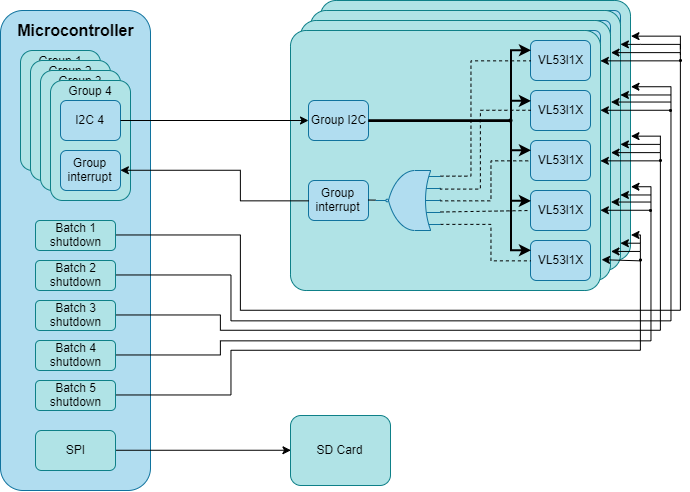
\includegraphics[width=100mm, keepaspectratio]{figures/data_collector.png}
    \caption{Design of data collector}
    \label{fig:data_collector}
\end{figure}

